\documentclass[12pt,a4paper]{article}
%\usepackage[utf8]{inputenc}
%\usepackage[portuguese]{babel}
\usepackage{amsmath, amsfonts, amssymb, mathrsfs}
\usepackage{graphicx}
\usepackage{newtxmath}
\usepackage[utf8]{inputenc} % Permite utilizar caracteres especiais: Ex: ç á à...
\usepackage[onehalfspacing]{setspace} % Espaçamento de 1,5
\usepackage{cabecalho}
\usepackage{float}
\usepackage{multirow}
\usepackage[lmargin=3cm, tmargin=3cm, rmargin=2cm, bmargin=2cm]{geometry}
\usepackage{indentfirst}
\usepackage{graphicx}
\usepackage[caption=false]{subfig}
% \usepackage[brazilian]{babel} % Traduzir para PT-BR
\usepackage{IEEEtrantools}
\usepackage{xcolor}
\usepackage[linesnumbered,ruled,vlined]{algorithm2e}
\interfootnotelinepenalty=10000
% Alguns comas
\newcommand{\rxy}{{\mathit{\mathbf{R}}}_{\mathit{x\mathbf{y}}}}
\newcommand{\ry}{{\mathit{\mathbf{R}}}_{\mathit{\mathbf{y}}}}
\newcommand{\wo}{\mathit{\mathbf{w_o}}}
\newcommand{\wn}{\mathit{\mathbf{w}}\left\lbrack n\right\rbrack}
\newcommand{\vn}{\mathit{\mathbf{v}}\left\lbrack n\right\rbrack}
\newcommand{\trans}{\mathsf{T}}
\newcommand{\hermit}{\mathsf{H}}
\newcommand{\mc}[1]{\ensuremath{\mathcal{#1}}}
\newcommand{\mbb}[1]{\ensuremath{\mathbb{#1}}}
\newcommand{\Natural}{\mathbb{N}}
\newcommand{\Integer}{\mathbb{Z}}
\newcommand{\Irrational}{\mathbb{I}}
\newcommand{\Rational}{\mathbb{Q}}
\newcommand{\Real}{\mathbb{R}}
\newcommand{\Complex}{\mathbb{C}}

\newcommand\mycommfont[1]{\footnotesize\ttfamily\textcolor{blue}{#1}}
\SetCommentSty{mycommfont}
\SetKwInput{KwInput}{Input}                % Set the Input
\SetKwInput{KwOutput}{Output}              % set the Output

\begin{document}
	\initcab{Universidade Federal do Ceará}{Inteligência Computacional Aplicada}{Guilherme Barreto and Ajalmar}{519024}{Junho/2022}{Neural network - Report}

\section{Work 01 - Rosenblatt's perceptron}

This work considers a classification problem for a multivariate dataset. The Rosenblatt's perceptron is utilized to classify the iris flower dataset. The problem consist in classifying one class among four subspecies (Setosa, Virginica, and Versicolor).

The Rosenblatt's perceptron comprises a neuron mathematical model, introduced by McCulloch and Pitts in 1943, with a learning algorithm that adjusts the synaptic weights in a supervised fashion. The McCulloch and Pitts' activation function is a step function that triggers the output from 0 to 1 when the induced local field overpass the threshold. This method is effective for binary classification of linearly separable problems, where one can sketch a straight line that divides the classes without overlapping.

At the instant \(n\), the induced local field is given by
\begin{align}
    v(n) = \mathbf{w}^\trans\left(n\right) \mathbf{x}\left(n\right),
    \label{eq:induced-local-field}
\end{align}

where \(\mathbf{w}^\trans\left(n\right) = \begin{bmatrix}
    w_0(n) & w_1(n) & \cdots & w_{N_a}(n)
\end{bmatrix}^\trans\) and \(\mathbf{x}^\trans\left(n\right) = \begin{bmatrix}
    x_0(n) & x_1(n) & \cdots & x_{N_a}(n)
\end{bmatrix}^\trans\) are the synaptic weights of the perceptron and the input signal, respectively, and \(N_a\) indicates the number of attributes. The elements \(w_0(n)\) and \(x_0(n) \triangleq +1\)\footnote{Depending on the author, it can the defined as \(-1\).} are, respectively, the bias and its input.

The machine learning algorithms settles on the well-established theory of adaptive filters. Particularly for the Rosenblatt's perceptron, it is utilized the Least-Mean-Square (LMS) algorithm, that aims to make a instantaneous approximation of the gradient vector. The optimization algorithm is given by
\begin{align}
    \mathbf{w}(n+1) = \mathbf{w}(n) - \eta \mathbf{g}(n),
    \label{eq:w_n+1}
\end{align}
where \(\eta\) is the step-learning hyperparameter and \(\mathbf{g}(n) \triangleq \nabla \mathscr{E} (\mathbf{w})\) is the stochastic approximation of the gradient vector, being \(\mathscr{E} (\mathbf{w})\) the cost function. The Equation \eqref{eq:induced-local-field} passes through the step function, \(\varphi \left( \cdot \right)\), generating the perceptron output, \(y\left( n \right) = \varphi(v\left( n \right)) \in \left\{ 0,1 \right\}\). This signal is compared to the desired value, \(d\left( n \right) \in \left\{ 0,1 \right\} \) and produces the error signal \(e\left( n \right) = d\left( n \right) - y\left( n \right) \in \left\{ -1, 0, 1 \right\}\), which indicates whether the perceptron misclassified or not. The LMS algorithm uses the instantaneous value of the MSE (Mean-Squared Error) cost function, that is,
\begin{align}
    \mathscr{E} (\mathbf{w}) = \frac{1}{2}e^2(n).
\end{align}
Differentiating this equation with respect to the synaptic weights, we get
\begin{align}
    \mathbf{g}(n) = \frac{\partial\mathscr{E} (\mathbf{w})}{\partial \mathbf{w}(n)} = - \mathbf{x}(n) e(n).
    \label{eq:g_n}
\end{align}
Substituting \eqref{eq:g_n} into \eqref{eq:w_n+1}, it yields the learning equation, given by
\begin{align}
    \mathbf{w}(n+1) = \mathbf{w}(n) + \eta \mathbf{x}(n) e(n).
    \label{eq:g_n}
\end{align}

The Algorithm \ref{alg:rosenblatt-perceptron} summarizes the procedure utilized for the Rosenblatt's perceptron, including data preparation techniques, such as hand-out and shuffling the dataset. The method utilizes \(N_r=20\) independent realizations, and passes through the training set \(N_e=100\) epochs. At the end of each realization, it is stored the accuracy reached by the test data, and the accuracy of all realizations are investigated in terms of mean and standard deviation. The iris dataset contains \(N=150\) instances with \(N_a=4\) attributes (petal length, petal width, sepal length, and sepal width) and \(K=3\) classes (Setosa, Versicolour, and Virginica). It was chosen a ratio of \(80\%-20\%\) for the training and testing dataset, respectively.

\begin{algorithm}[!ht]
    \DontPrintSemicolon
      
      \KwInput{\(\mathbf{X}, \mathbf{d}\) \tcc*{attributes and labels dataset}}
      
    %   \KwData{Testing set $x$}
      \ForAll{\(\left\{ 1, 2, \cdots, N_r \right\}\)}{
        \(\mathbf{w}(n) \leftarrow \text{initialize}\)

        \(\mathbf{X}, \mathbf{d} \leftarrow \text{shuffle}\)

        \( \left( \mathbf{X}_{trn}, \mathbf{d}_{trn} \right), \left( \mathbf{X}_{tst}, \mathbf{d}_{tst} \right)  \leftarrow \text{hold-out}\) \tcc{training and testing dataset}

        \ForAll{\(\left\{ 1, 2, \cdots, N_e \right\}\)}{
            \ForAll{Instancies in the training dataset}{
                \(v(n) \leftarrow \mathbf{w}^\trans\left(n\right) \mathbf{x}\left(n\right)\)

            \(y\left( n \right) \leftarrow \varphi(v\left( n \right))\)

            \(e(n) \leftarrow d\left( n \right) - y\left( n \right)\)

            \(\mathbf{w}(n+1) \leftarrow \mathbf{w}(n) + \eta \mathbf{x}(n) e(n)\)
            }
            \(\mathbf{X}_{trn}, \mathbf{d}_{trn} \leftarrow \text{shuffle}\)
        }
        
        \(accuracy \leftarrow \text{test}(\mathbf{X}_{tst}, \mathbf{d}_{tst})\)
      }
    
    \caption{Rosenblatt's perceptron}
    \label{alg:rosenblatt-perceptron}
\end{algorithm}

The process described in Algorithm \ref{alg:rosenblatt-perceptron} was repeated for each class and results are shown in Table \ref{tab:rosenblatt-results}. The setosa class clearly outperforms other classes since it is linearly separable for some attributes, as shown in the decision surface in Figure \ref{fig:rosenblatt-decision-surface}\footnote{Since the problem has four attributes, this plot would be impossible as the would get 2 degree of freedom. Therefore, for this result, we considered only the two attributes showed in the figure.}.

\begin{figure}[H]
    \centering
    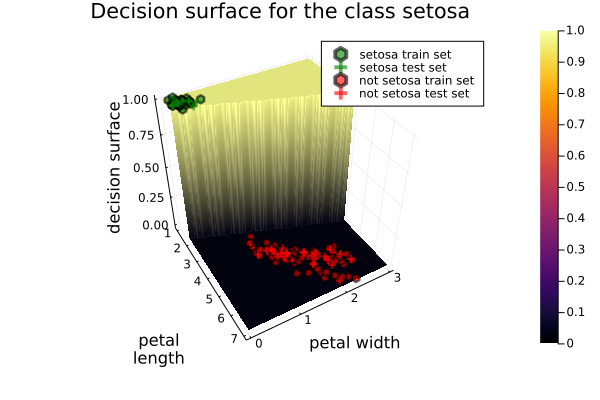
\includegraphics[scale=0.35]{../trab1 (simple perceptron)/figs/decision-surface-for-setosa.png}
    \caption{Decision surface of setosa class.}
    \label{fig:rosenblatt-decision-surface}
\end{figure}

\begin{table}
	\centering
	\caption{Rosenblatt's perceptron performance for classification problem}
	\footnotesize
	\setlength{\tabcolsep}{5pt}
	\begin{tabular}{ccccccccc}
		% \toprule [1.3pt]	
		% \multicolumn{4}{c}{ \textbf{Style} } \\
		\hline
		Classes & mean accuracy & standard deviation \\
		\hline
		Setosa & 98.33 & 0.01972 \\
        \hline
		Virginica & 54.16 & 0.1251 \\
		\hline
		Versicolor & 53.66 & 0.1591 \\
		\hline
	\end{tabular} \label{tab:rosenblatt-results}
\end{table}

The confusion matrix of the setosa class is shown in Figure \ref{fig:confusion-matrix-setosa} for the first realization. The main diagonal indicates that there were neither false negative nor false positive.

\begin{figure}[H]
    \centering
    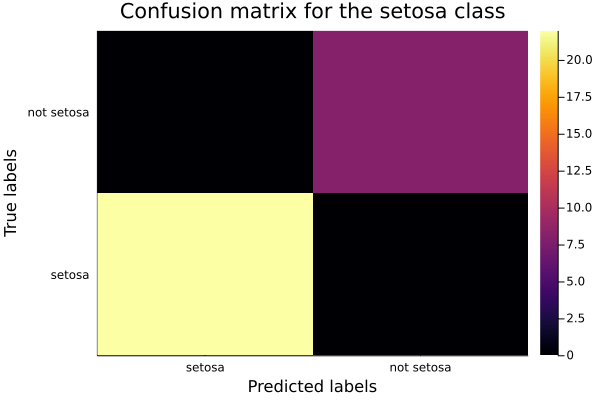
\includegraphics[scale=0.35]{../trab1 (simple perceptron)/figs/setosa-confusion-matrix.png}
    \caption{confusion matrix for setosa class.}
    \label{fig:confusion-matrix-setosa}
\end{figure}

The Figure \ref{fig:setosa-training-evolution} shows the evolution of the training dataset accuracy throughout the epochs. One can notice the fast convergence to accuracy of 100\%.

\begin{figure}[H]
    \centering
    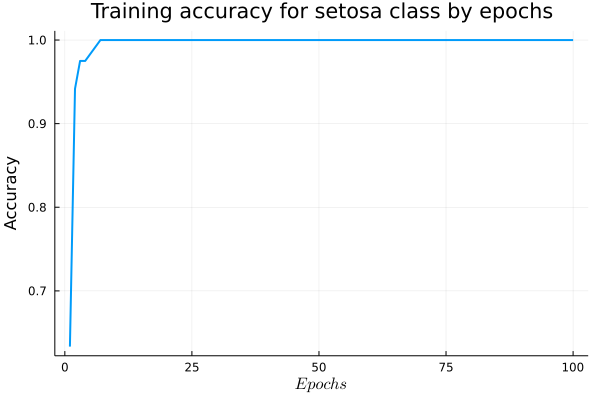
\includegraphics[scale=0.35]{../trab1 (simple perceptron)/figs/accuracy-by-epochs-for-setosa.png}
    \caption{Training dataset evolution for the setosa classification.}
    \label{fig:setosa-training-evolution}
\end{figure}

For a dummy dataset with \(K=4\) classes, the Rosenblatt's perceptron achieved a mean accuracy of 97.5\% and a standard deviation of 0.05. The Figure \ref{fig:decision-surface-dummy-data} shows the decision surface of the desired class for the realization whose accuracy the closest to the mean accuracy. All instances of all classes are samples drawn from a Gaussian distribution with a given mean and variance.

\begin{figure}[H]
    \centering
    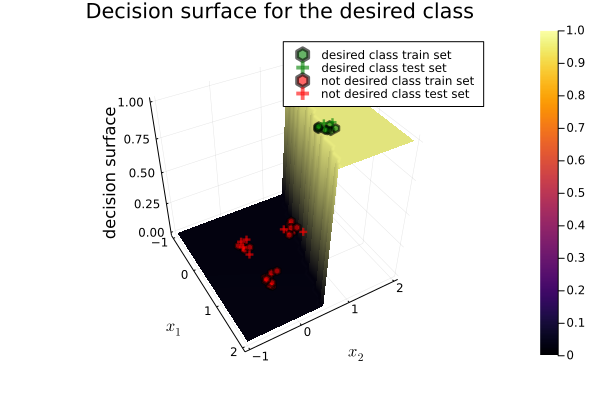
\includegraphics[scale=0.35]{../trab1 (simple perceptron)/figs/decision-surface-for-dummy-data.png}
    \caption{Decision surface for the desired class.}
    \label{fig:decision-surface-dummy-data}
\end{figure}

\section{ADALINE}

The Adaptive Linear Element (or ADALINE) is a variation of the Rosenblatt's perceptron, where the step function is replaced by a linear function, that is, \(y(n) = \varphi(u(n)) = u(u)\). One can combine a tapped delay line with an ADALINE, thus creating an adaptive filter, widely used in statistical signal processing.

Consider a regression problem where the desired signal comes from a function \(f(x)\) corrupted with a Gaussian noise. The ADALINE model tries to retrieved the original data using the same process described in Algorithm \ref{alg:rosenblatt-perceptron}. However, the performance analysis is around the MSE error instead the accuracy since it is now a regression problem.

The Table \ref{tab:adaline-results} shows the performance of the mean MSE and its standard obtained over the independent realizations, in addition the root mean squared error (RMSE). We considers two scenarios for the \(f (x)\): linear and quadratic function.

\begin{table}[H]
	\centering
	\caption{ADALINE performance for regression problem}
	\footnotesize
	\setlength{\tabcolsep}{5pt}
	\begin{tabular}{ccccccccc}
		% \toprule [1.3pt]	
		% \multicolumn{4}{c}{ \textbf{Style} } \\
		\hline
		\(d(n)\) & MSE mean & MSE standard deviation & RMSE mean & RMSE standard deviation \\
		\hline
		\(5x+8\) & 13.17 & 4.69 & 3.57 & 0.65  \\
        \hline
		\(0.5x^2+3x+6\) & 281.85 & 131.4 & 16.41 & 3.5 \\
		\hline
	\end{tabular} \label{tab:adaline-results}
\end{table}

Naturally, the linear function achieved the best result since ADALINE can effectively solve a linear problem. Indeed, the synaptic weights of the ADALINE model is close to the coefficients of the linear function, \(\mathbf{w} = \begin{bmatrix}
    -6.8 & 4.977
\end{bmatrix}\)\footnote{The negative value it is because it was chosen an input bias of \(x_0(n)=-1\).}. The Figure \ref{fig:ADALINE-regression} shows the regression for the ADALINE model.

\begin{figure}[htp]
    \centering

\subfloat[\centering ADALINE regression for \(5x+8\)]{%
  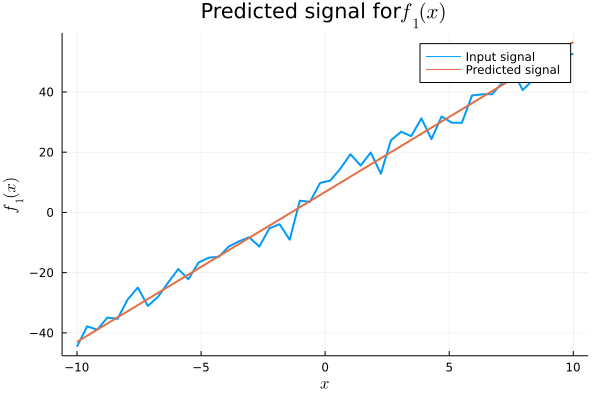
\includegraphics[clip,scale=0.4]{../trab2 (ADALINE)/figs/predict-f1.png}%
  \label{fig:itema}
}

\subfloat[\centering ADALINE regression for \(0.5x^2+3x+6\)]{%
  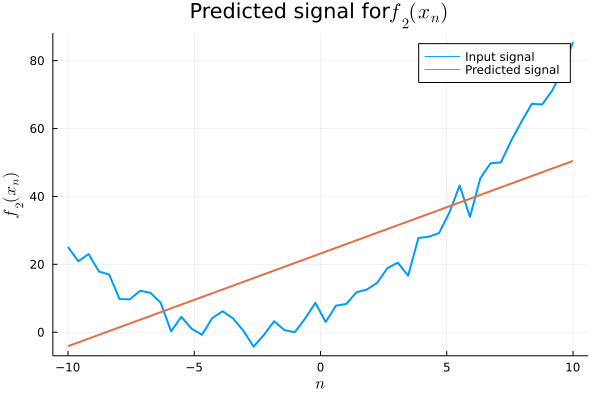
\includegraphics[clip,scale=0.4]{../trab2 (ADALINE)/figs/predict-f2.png}%
  \label{fig:itemb}
}

\caption{ADALINE regression}
\label{fig:ADALINE-regression}

\end{figure}

\section{Single Layer Perceptron}

Although Rosenblatt's perceptron can solve linear problems, it has only one output variable. A more reasonable model for a multivariate class problem is a single-layer perceptron consisting of \(K\) neurons, where each neuron receives the same input signal, \(\mathbf{x}(n)\).

The matrix of all coefficients is given by
\begin{align}
    \mathbf{W}(n) = \begin{bmatrix}
        \mathbf{w}_1 (n) & \mathbf{w}_2 (n) & \cdots & \mathbf{w}_K (n)
    \end{bmatrix} \in \Real^{K \times N_a+1},
\end{align}
where \(K\) is the number of classes (a neuron for each class) and \(N_a\) is the number of attributes. The learning algorithm is given by
\begin{align}
    \mathbf{W}(n+1) = \mathbf{W}(n) + \eta \boldsymbol{\deltaup}(n) \mathbf{x}(n)^\trans,
\end{align}
where \(\boldsymbol{\deltaup}(n) = \begin{bmatrix}
    \delta_1(n) & \delta_2(n) & \delta_K(n)
\end{bmatrix}^\trans\) is the vector of the local gradients, being \(\delta_k(n) = e_k (n) \varphi'(v_k (n))\) the local gradient of the \(k\)th perceptron, and \(\varphi'(v_k (n))\) is the derivative of output activation function, \(\varphi(v_k (n))\), with respect to \(v_k (n)\). For the step function (MacCulloch and Pitts' activation function), its derivative does not exist, and the local gradient of the \(k\)th neuron is simply \(\delta_k(n) = e_k (n)\). For this classification problem, the labels was encoded using the one-hot method.

The Figure \ref{fig:heatmap-dummy-dataset} shows the heatmap for a dummy dataset consisting of \(K=3\) classes, \(N_a=2\) attributes, and \(N=150\) instances. The classifier used the MacCulloch and Pitts' activation function and achieved a mean accuracy of 99.49\% and a standard deviation of 0.0218. The same classifier was used for the iris dataset (\(K=3\) classe, \(N_a=4\) attributes, and \(N=150\) attributes) and the column dataset (\(K=3\) classes, \(N_a=6\) attributes, and \(N=310\) instances). For the iris dataset, the classifier achieved a mean accuracy of 88\% with a standard deviation of \(0.14\), while for the column dataset the model achieved mean accuracy of 77.66\% with a standard deviation of \(0.06\).

\begin{figure}[H]
    \centering
    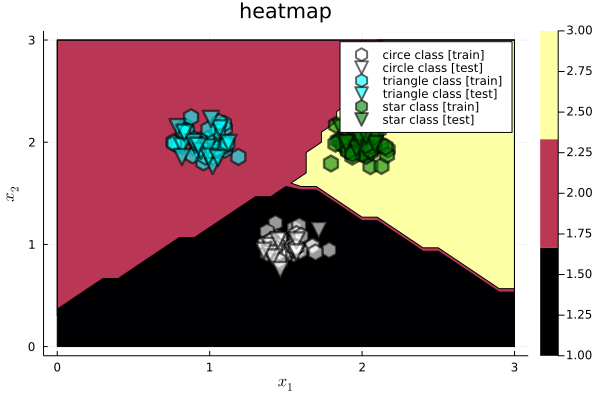
\includegraphics[scale=0.5]{../trab3 (single layer perceptron)/figs/dummy data - heatmap.png}
    \caption{Heatmap of the dummy dataset.}
    \label{fig:heatmap-dummy-dataset}
\end{figure}

Using the signal function, the model achieved a mean accuracy of 100\% for the dummy data. The surface of decision for each class of iris data is shown in Figure \ref{fig:iris-decision-surface}. It is possible to notice that the classifier can successively solve the problem for the setosa class as it is linearly separable from the other classes for the attributes considered (petal length and petal width).

\begin{figure}[tp]
    \centering
    \subfloat[\centering Setosa class]{%
      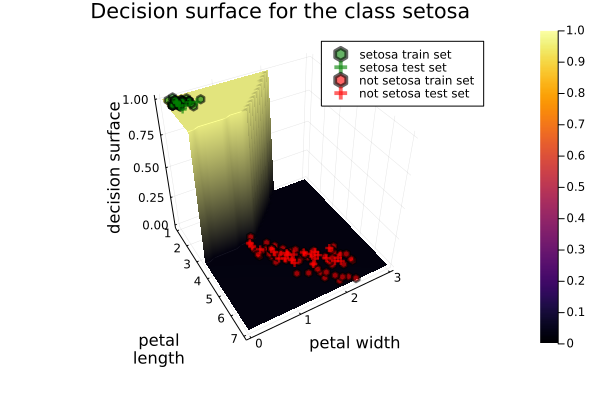
\includegraphics[scale=0.4]{../trab4 (single layer perceptron with sigmoidal functions)/figs/decision-surface-for-setosa.png}%
    }
    
    \subfloat[\centering Verginica class]{%
      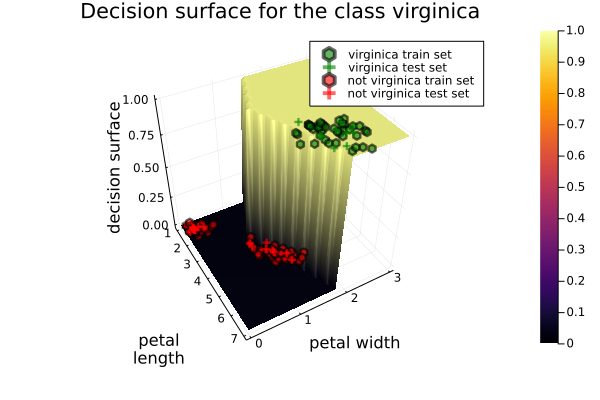
\includegraphics[scale=0.4]{../trab4 (single layer perceptron with sigmoidal functions)/figs/decision-surface-for-virginica.png}%
    }

    \subfloat[\centering Versicolor class]{%
      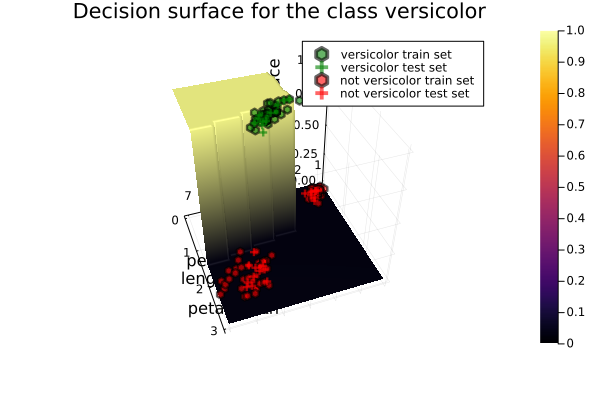
\includegraphics[scale=0.4]{../trab4 (single layer perceptron with sigmoidal functions)/figs/decision-surface-for-versicolor.png}%
    }
    
    \caption{main caption}
    \label{fig:iris-decision-surface}
    
    \end{figure}

\end{document}